\documentclass{qor-eume-ext-abstract}

\title{Author Instructions for Submitted Extended Abstracts}
\shorttitle{Template}

\author[1]{Alexey Bochkarev}
\author[2]{Caroline Prodhon}
\shortauthors{A.\ Bochkarev, C.\ Prodhon}

\affilblock[1]{RPTU Kaiserslautern-Landau,\par Gottlieb-Daimler-Straße 31,
67663 Kaiserslautern\par\href{mailto:a.bochkarev@rptu.de}{a.bochkarev@rptu.de}}
\affilblock[2]{Université de Technologie de Troyes,\par 12 rue Marie Curie, CS 42060, 10004 Troyes CEDEX\par\href{mailto:caroline.prodhon@utt.fr}{caroline.prodhon@utt.fr}}

\date{2025/04/25}

% your bibliography file
\addbibresource{refs.bib}

\begin{document}

\maketitle

\section{Introduction}
You will find here the basic instructions to prepare your paper for submission
to the Joint meeting of the EURO Working Groups for Metaheuristics and Quantum
OR in 2025.

\section{Author instructions}
The extended abstacts for submission must follow the instructions below.

\begin{itemize}
  \item Language: English
  \item The formatting is set in the \texttt{qor-eume-ext-abstract} class.
        Please refer to the source code of this file (\texttt{example.tex}) for
        the usage details.
  \item Page limit: 6 pages. You will see a warning on compilation if you exceed
        it, but the limit is not strict. Therefore, please do not try to reduce
        the number of pages, e.g., by using 10pt font size or changing the text height,
        the text width or the margins.
  \item For submission deadlines and further details please refer to the event
        website:
        \begin{center} \href{https://perso.isima.fr/~lacomme/EUME_JE2/EUME_Joint_Event.php}{https://perso.isima.fr/\~lacomme//EUME\_JE2/EUME\_Joint\_Event.php}
        \end{center}
\end{itemize}

\subsection{Figures}
Please use the standard \texttt{figure} environment, with centering and placing
the caption below the figure, like we did with \cref{fig:example}. We rely on
the figure placement done by \LaTeX, but try to have the figures reasonably
close to where they are cited. (We used \texttt{[H]} option of the
\texttt{\\figure} environment here.)

\begin{figure}[H]
  \centering
  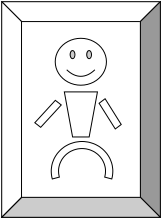
\includegraphics{figures/figure.png}
  \caption{An example of a figure.\label{fig:example}}
\end{figure}

\subsection{Tables}
Please use \texttt{booktabs} \LaTeX package, with centered tables and a caption
above, as we do with the example in \cref{tab:example}.

\begin{table}[H]
  \centering
  \caption{An example of a table.\label{tab:example}}
  \begin{tabular}{ccc}
    \toprule
    Column 1 & Column 2 & Column 3\\
    \midrule
    2 & 3 & 1\\
    4 & 5 & 9\\
    \bottomrule
  \end{tabular}
\end{table}

Similarly to figures, we rely on the placement done by \LaTeX, but try to have
the tables reasonably close to where they are cited. (Here we used the
\texttt{H} option to achieve this.)

\subsection{References}
References should appear in a separate section at the end of the document. They
must be complete, accurate, and listed in alphabetical order of the last name of
the first author.\vspace{\baselineskip}

When quoted, a reference should appear as a number: for instance,
\cite{sorensen2006} or \cite{bochkarev2024}.

\printbibliography

\end{document}

%%% Local Variables:
%%% mode: LaTeX
%%% TeX-master: t
%%% End:
